\documentclass[conference, compsoc]{IEEEtran}
%\documentclass[letter,11pt]{article}
%\documentclass[letter,10pt]{scrartcl}

\usepackage[utf8]{inputenc}
\usepackage[pass,letterpaper]{geometry}
\usepackage{graphicx}
\usepackage{listings}
\usepackage{color}
\usepackage{float}
\usepackage{bigfoot}
%\usepackage[square,sort,comma,numbers]{natbib}
%\usepackage{titling}
%\usepackage{mathtools}
\usepackage{helvet}
\usepackage{algorithmicx}
\usepackage{algpseudocode}

\ifCLASSOPTIONcompsoc
  % IEEE Computer Society needs nocompress option
  % requires cite.sty v4.0 or later (November 2003)
  \usepackage[nocompress]{cite}
\else
  % normal IEEE
  \usepackage{cite}
\fi


\setlength{\parindent}{0cm}



\pdfinfo{%
  /Title    (OpenMemDB: A wait-free database)
  /Author   (Mike McGee, Neil Moore, Robert Medina, Jason Stavrinaky)
  /Creator  ()
  /Producer ()
  /Subject  ()
  /Keywords ()
}

\let\oldReturn\Return
\renewcommand{\Return}{\State\oldReturn}

\newcommand{\CC}{C\nolinebreak\hspace{-.05em}\raisebox{.4ex}{\tiny\bf +}\nolinebreak\hspace{-.10em}\raisebox{.4ex}{\tiny\bf +}}


\definecolor{codegreen}{rgb}{0,0.6,0}
\definecolor{codered}{rgb}{0.6,0,0}
\definecolor{codegrey}{gray}{0.9}

\newcommand{\inlinecode}[1]{\colorbox{codegrey}{\lstinline[language=C++]{#1}}}

\begin{document}

\title{OpenMemDB: A wait-free database\thanks{Sponsor: Dr. Damian Dechev}}
\author{
\IEEEauthorblockN{Michael McGee} \and 
\IEEEauthorblockN{Robert Medina} \and 
\IEEEauthorblockN{Neil Moore} \and 
\IEEEauthorblockN{Jason Stavrinaky}
}

\date{2/1/2016}

\pagenumbering{gobble}
\maketitle
\newpage

\pagenumbering{arabic}
\begin{abstract}
OpenMemDB is an in-memory database that is implemented using solely wait-free
data structures. OpenMemDB is the first and only database currently developed in such a
way. OpenMemDB also provides linearizable correctness guarantees for all operations
executed on the database. OpenMemDB uses a form of snapshot isolation to ensure 
linearizability, and avoids the write-skew problem that can occur when using
snapshot isolation by eliminating writes that are out of data. 
OpenMemDB's biggest contribution is it's completely wait-free 
implementation. Every operation executed in OpenMemDB is guarenteed to be wait-free 
and linearizeably correct. This implementation also scales extremely well, and performs 
{{ENTER PERCENT HERE}} better than similar in-memory database management systems.
{{NEED A LITTLE BIT MORE ABOUT THE PERFORMANCE}}
\end{abstract}

\section{Introduction}
While hard drives are getting faster due to the introduction of NAND flash-based drives,
they are still relatively slow when compared to main memory. Meanwhile main memory is 
following a long running pattern where it has precipitously dropped in price from costing 
thousands of dollars for a few megabytes to about \$40 for 8 gigabytes \cite{jcmit}. 
With this trend, we can take advantage and design fast databases that reside entirely in main memory. While the largest of datasets are still too large for main memory, 
some datasets are finally able to fit into main memory in modern systems due to the 
cheapness and advancement of memory module technology. 
\par\vspace{\baselineskip}
Most technologies have advanced 
along with hardware, however database management systems have struggled to improve
at a similar rate. This is mostly due to concurrency issues. Databases spend more than 30\% 
of execution time in synchronization-related operations, even when only running a single
client thread\cite{soares2015database}. And in this era, where a powerful server
can have more than a terabyte of RAM and well over 64 cores, effectively utilizing all of 
this processing power is essential. 
\par\vspace{\baselineskip}
Our approach, OpenMemDB, solves this problem by implementing a data-store 
using only wait-free data structures that scale extremely well with added cores. 
OpenMemDB is a SQL database designed from the ground up to provide fast access to shared
data without using any locks. This is achieved through the use of wait-free
data-structures provided by Tervel, a library of wait-free and lock-free data-structures
developed by Feldman et. al\cite{tervel:hazard_pointer}\cite{tervel:hash_map}\cite{tervel:vector}. The lack of contention on locks and the wait-free
guarantees that the Tervel data-structures provide will achieve the performance gains that 
have been lacking in the DBMS field. 
\par\vspace{\baselineskip}
OpenMemDB's biggest contribution is in being the first completely wait-free database 
management system. Wait-freedom is a progress guarantee for concurrent data-structures 
which states that all threads running operations on the data-structure are guaranteed 
to complete in a finite number of steps. This sort of guarantee can be vital in 
real-time systems where a hard limit needs to be placed on how long an operation 
is allowed to take. One situation in which OpenMemDB would be ideal is for use in real-time 
database systems, where data has a temporal validity, and all calculations using this data 
must complete within this valid range of time. An example of a real-time database system 
is a stock market analysis database. A database that is used to track the current state
of the stock market and run calculations based on the temporarily valid data. 
\par\vspace{\baselineskip}
OpenMemDb
is also well suited for any situation in which a large amount of calculations need to be 
executed on a relatively centralized data-set. This is due to the fact that OpenMemDB 
provides all threads access to every part of the database. Some database systems attempt to 
use data partitioning to help parallelize their operations, these systems would not be a 
good choice if the data-set could not be efficiently partitioned. OpenMemDB does not do any 
partitioning and still manages to achieve {{INSERT SCALING HERE}} scaling. 
\par\vspace{\baselineskip}
OpenMemDB also 
retains all necessary ACID properties, which is vital for most database systems. 
The requirements of being wait-free dictate that 
OpenMemDB is an in-memory database and thus avoids the bottlenecks associated with 
going to hard disk. OpenMemDB is written in \CC 11 and uses the modern constructs defined by 
that standard extensively.
\par\vspace{\baselineskip}

\section{Related Work}
There are several other in-memory database management systems that attempt to solve the 
problem of data-contention. This being the main source of slow downs for in-memory systems.

The database management system most related to OpenMemDB is MemSQL.
MemSQL uses lock-free data structures for every component of their database management
system. MemSQL uses lock-free skips lists and hash tables for the bulk of their data-store\cite{MemSQL}.
They also use MVCC (Multi-version Concurrency Control) to provide fast transactions. 
OpenMemDB does something similar with snapshot isolation. MemSQL also compiles SQL
statement to C++ code and stores this code to be used if the SQL statement is ever called
again. Something that OpenMemDB does not implement.

VoltDB is an in-memory database management system that uses pure SQL, is completely ACID
compliant, and does not use locks. They claim to achieve 100 times the performance of 
a traditional relation database management system, with near linear scaling with added nodes \cite{voltdb2010voltdb}. They claim to achieve 560,000 transaction per second on a 12
partition set up. 
VoltDB uses a shared nothing architecture. Their execution engine is single threaded, 
avoiding the overhead of locking or latching \cite{voltdb2010voltdb}. This requires
intelligent partitioning of data and does not allow for multi-threaded execution 
on a single partition. 

Silo is an in-memory database that uses optimistic concurrency control (OCC) to try and 
limit the affects of locks on their system. Silo avoids locking during the computation
of a transaction and waits until commit time to execute all writes to shared memory.
This avoids the contention involved in acquiring a lock until a short period of time 
at the end of transaction. This style of system can be particularly effective if
concurrent writes to shared memory are uncommon. Silo claims to achieve 700,000
transaction per second an a 32 core machine. Silo relies heavily on concurrent 
B+ tree for its back end data-store \cite{tu2013speedy}. 

Hekaton is Microsoft's main memory optimized database engine.
Hekaton uses a combination of lock-free data-structures and optimistic concurrency control
in order to achieve scaleable performance gains. Hekaton is like Silo and OpenMemDB in that 
it does not use partitioning to achieve performance gains. Any thread can access any 
row in a table without acquiring a lock\cite{diaconu2013hekaton}. Hekaton claims to gain
an order of magnitude performance gain over standards SQL Server\cite{diaconu2013hekaton}

%TODO fix the rest of this
%MemSQL\footnote{MemSQL can be configured as a Columnstore that stores data on disk.}
%and VoltDB are both fully in-memory DBMS as is OpenMemDB. This is where the
%similarities end as far as OpenMemDB is concerned. MemSQL and VoltDB on the other 
%hand both use distributed systems to achieve performance gains and they both differ from 
%OpenMemDB in a few ways. MemSQL uses lock-free data structures
%to store data and stores pre-compiled commonly used queries\cite{MemSQL}.
%VoltDB tries to make its performance gains by what they call Concurreny through
%scheduling\cite{VoltDB}. This is the process of using a single-threaded pipeline 
%that performs the task it was scheduled. This limits the need for locking during
%transactions by intelligently scheduling the transactions so that locks are not
%necessary. This approach eliminates the time spent obtaining and updating a lock
%but limits parallelization. There can not be true concurrent access on shared data. If 
%there are a number of operations that need to be executed on the same table in a database; 
%these operations will be scheduled sequentially. The only parallelism that occurs is during
%operations on unrelated data. Our approach allows for concurrent operations to take place
%no matter what data is being accessed.

\section{Technical Approach}
Our database is built upon wait-free data structures found in Tervel, a collection of
lock-free and wait-free data structures created by Steven Feldman, Pierre LaBorde, and Damian Dechev\cite{tervel:hazard_pointer}\cite{tervel:hash_map}\cite{tervel:vector}. 
We use the common definition of wait-freedom as found in Herlihy's definitive text, which
states that all threads must make progress within a finite amount of time\cite{herlihy:waitfree}.
We also use the statement that a composition of linearizable algorithms or data structures
is also linearizable. From the beginning, we knew that we had to compose 
the linearizable and wait-free components given to us. Using that composition 
as the sole shared object and thus the sole way to communicate 
between the threads within the system ensures that we are indeed linearizable.
From there we can then prove that all running threads are guaranteed 
to make progress in some finite time and thus prove wait-freedom from that foundation.
\par\vspace{\baselineskip}
The architecture of our database is simple, with three main modules that 
communicate with each other: the Work Manager, SQL Engine, and Data Store.
Each module has a distinct responsibility and mechanism of fulfilling that responsibility with as 
little communication between threads as possible. The Work Manager is responsible for distributing
incoming queries and commands among the worker threads as well as sending the results back to the 
client that sent them. The SQL Engine is responsible for parsing the
given query or command string into an internal representation that can be executed on the Data Store.
The Data Store is where all the database's data is stored and thus is where the wait-free data
structures are primarily used. These wait-free data structures are used so that all
the worker threads can safely and efficiently execute their assigned tasks. The guarantees of a 
wait-free data structure are such that multiple threads can work on the same data without 
running into concurrency conflicts within the data structures or waiting on another thread to 
finish for an indeterminate amount of time. Once the threads calculate their results, they 
send those results to the Work Manager.
\par\vspace{\baselineskip}
Each worker thread is a long-lived thread spawned by the database upon start-up 
and has various thread-local statically-allocated pieces of memory given to it.
This memory is used by the parser within the SQL Engine module and helps keep the amount
of shared memory near zero. When the thread leaves the SQL Engine and proceeds to 
execute the parsed statement, it calls the appropriate method within the Data Store 
module. In this module the data structures and algorithms' wait-freedom and linearizability 
guarantees provide a fast and efficient way to create, modify, and access the stored data.  
We specifically use a wait-free hash map to relate table names to the tables themselves 
which are nested wait-free vectors. The composition of the Tervel vectors to create 
the table structure is that the outer vector acts as a container of references 
to records within the table while each of the referenced vectors contain the stored 
data. Access to these data structures is minimized to reduce code complexity and 
possible contention between threads over the data contained in the structures.
\par\vspace{\baselineskip}
Specifically, the Data Store methods used by the worker threads make local copies of 
the data contained in the core data structures as much as possible so as to take 
advantage of the standard library's well-defined and optimized containers. This also 
allows us to concretely define the situations where multiple writers attempt to write 
to the same element in the shared data structures. In the few situations this can occur, 
namely in the event of multiple concurrent SQL UPDATE or DELETE statements, we only perform
the operation if the targeted record reference in the table vector has not been changed. 
This is done using Tervel's compare-and-swap operation on a particular element in the 
vector. A compare-and-swap operation is a swap operation that only occurs when a comparison 
with an expected value succeeds. Failing to perform this swap due to the selected 
record reference changing between the time of selection and the time to perform the operation 
is deemed a soft failure due to contention. That soft failure would be caused by concurrently
running statements that work on the same records. As such, these soft failures are communicated
back to the client for them to handle as they see fit.
\par\vspace{\baselineskip}
Handling two concurrent update operations that occur at the same time as a long-lived 
read operation is an edge case that OpenMemDB handles using Tervel's hazard pointer. A 
hazard pointer is a wait-free smart pointer that will only allow freeing of the pointer 
if there are no references to the pointer within the Tervel data structures. Extending 
the hazard pointer lets us replace a record within a table as described above while 
maintaining the validity of the reference used by the read operation until that read 
operation concludes and the replaced record is released.
\par\vspace{\baselineskip}
Inserting records into a table within the Data Store requires pre-processed data to be passed
into the \inlinecode{InsertRecord} method of the Data Store object. The general procedure of inserting
into a table is shown in Figure \ref{insert_record}. This method first retrieves the table 
that we want to insert into and ensures the data provided adheres to the schema defined 
at the table's creation. Assuming that check is successful, a Tervel vector is then 
constructed using the given data while preserving the order of the data. Once the vector 
is setup we then push the reference to the Tervel vector into the table.

\begin{figure}
 \begin{algorithmic}
 \Function{InsertRecord}{TableName, Data}
 \State{T = \Call{GetTable}{TableName}}
 \If{$\Call{SchemaCheck}{$T, D$}\neq True$}
  \Return{$False$}
 \EndIf
 \State{R is a Tervel vector}
 \ForAll{D in Data}
  \State\Call{PushBack}{R,D}
 \EndFor
 \State\Call{PushBack}{T,R}
 \Return{$True$}
 \EndFunction
 \end{algorithmic}
 \caption{How a record is inserted into a table in OpenMemDB}
 \label{insert_record}
\end{figure}

\par\vspace{\baselineskip}
Our handling of read-only operations is similar to the relativistic programming approach detailed 
in Howard and Walpole's paper on relativistic red-black trees, where each reader of the 
data structures only works within its own temporal frame of the data structure\cite{rbtree}. 
This is done by copying to local unshared memory and then manipulating the data, 
effectively capturing a snapshot of the data that we then use to generate the final 
output given to the client. The acquisition of the data is bounded and cannot 
infinitely loop or block because Tervel's algorithms provide wait-free access 
to the shared data structures. An example of this style of data manipulation is shown in 
Figure \ref{read_op}. That function searches the given table for records that match
the predicate supplied and then returns a copy of those records. A predicate is defined
as a binary tree where each leaf node is some sort of comparison operation on a column
within a record. For example, the statement \inlinecode{SELECT A.* FROM A WHERE A.x = 1 AND A.y = 2}
would have a predicate with three nodes where the two leaves are the comparisons
\inlinecode{A.x = 1} and \inlinecode{A.y = 2}. The \inlinecode{EvaluatePredicate} call
walks that tree and creates a final set of records that satisfies all of the
leaf nodes. Those copied records are then returned to the caller which will then
pass them back to the client that initially sent the request.

\begin{figure}[h]
 \begin{algorithmic}
 \Function{GetRecords}{TableName, Predicate}
 \State{$T\gets \Call{GetTable}{TableName}$}
 \State{$Result\gets empty\ vector$}
 \If{Predicate is null}
  \ForAll{records $R$ in $T$}
  \State{\Call{PushBack}{Result, R}}
  \EndFor
 \Else
  \State{$Result\gets \Call{EvaluatePredicate}{T, Predicate}$}
 \EndIf
 \Return{$Result$}
 \EndFunction
 \end{algorithmic}
 \caption{An example of a read operation done on the tables stored in the Data Store}
 \label{read_op}
\end{figure}

\par\vspace{\baselineskip}
There are particular scenarios when the effects of concurrent SQL statements must be reordered
in order to maintain a valid sequential history, particularly when SELECT or UPDATE operations
are interleaved with DELETE or DROP TABLE operations and the operations operate on the same 
records or tables in the database. An example concurrent history of this interleaving is shown in 
Figure \ref{concurrent_history}.

\begin{figure}[h]
\centering
  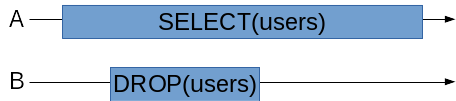
\includegraphics[scale=.75]{concurrent_history_1}
  \caption{A possible concurrent history that OpenMemDB must be able to linearize}
  \label{concurrent_history}
\end{figure}

\par\vspace{\baselineskip}
To properly linearize the history in Figure \ref{concurrent_history}, we need to reorder 
the effects of the DROP operation to take place after the SELECT. Using smart pointer features 
in the language chosen for this project, we can both postpone the deletion of the 
table data while completing the DROP operation. The smart pointer guarantees the memory will 
be deleted when all references to it are released, and as the base reference (stored in the 
relation of table name to table) is removed by the DROP operation, the operation's effects 
are effectively reordered to take place after the SELECT operation. This is similar to Tervel's 
hazard pointer functionality, but is simpler and only protects a single member in the object stored
in the hash map rather than the entire object. Furthermore, the smart pointer simply triggers a 
more fine-grained deletion of the table which then uses full Tervel protections to ensure memory
safety.

\section{Experimental Results}
PENDING

\section{Conclusions}
PENDING

\newpage
\bibliography{WorkshopPaper}
\bibliographystyle{acm}
\newpage

\end{document}
